\section{HXRM firmware}

Based on the results of research and simulations, the best timing
and shaping algorithms were implemented in hardware.
The ADQ14 uses Verilog and Vivado 2015.2, so these tools
were chosen for the implementation of the HXRM.
The developed system performs pulse detection,
measures the peak height, stores the resultant spectrum
and periodically transfer the results to the host PC.

\subsection{System overview}

As described in \autoref{ssec:adq_devkit} the ADQ14 DevKit
grants a semi-open FPGA design with two modules that can be
freely modified by the end user. The board manufacturer
designed User Logic 1 with intent for it to house timing filters
and User Logic 2 to contain more specialized processing logic.
Initially, these ideas were followed with a Boxcar filter being
implemented in User Logic 1 and a Pulse Height Analyzer being placed 
in User Logic 2.


With the default firmware, ADQ14 generates fixed-length records
on trigger events. For example, with the window length set to a 1000
samples, upon the detection of a pulse, 1000 samples would always be
transferred to the PC, irregardless of pile ups and other disturbances.
For this reason the timing logic originally placed in User Logic 1 was moved
to User Logic 2, so that it could be better integrated with the rest 
of the pulse analysis systems. The UL2 module allows for full control 
over record lengths so sampling windows in which pile ups were detected
could now be rejected, split into two or prolonged depending on the need.
\autoref{fig:firmware_overview} gives an overview of the system designed
in User Logic 2.

\begin{figure}[H]
  \centering
  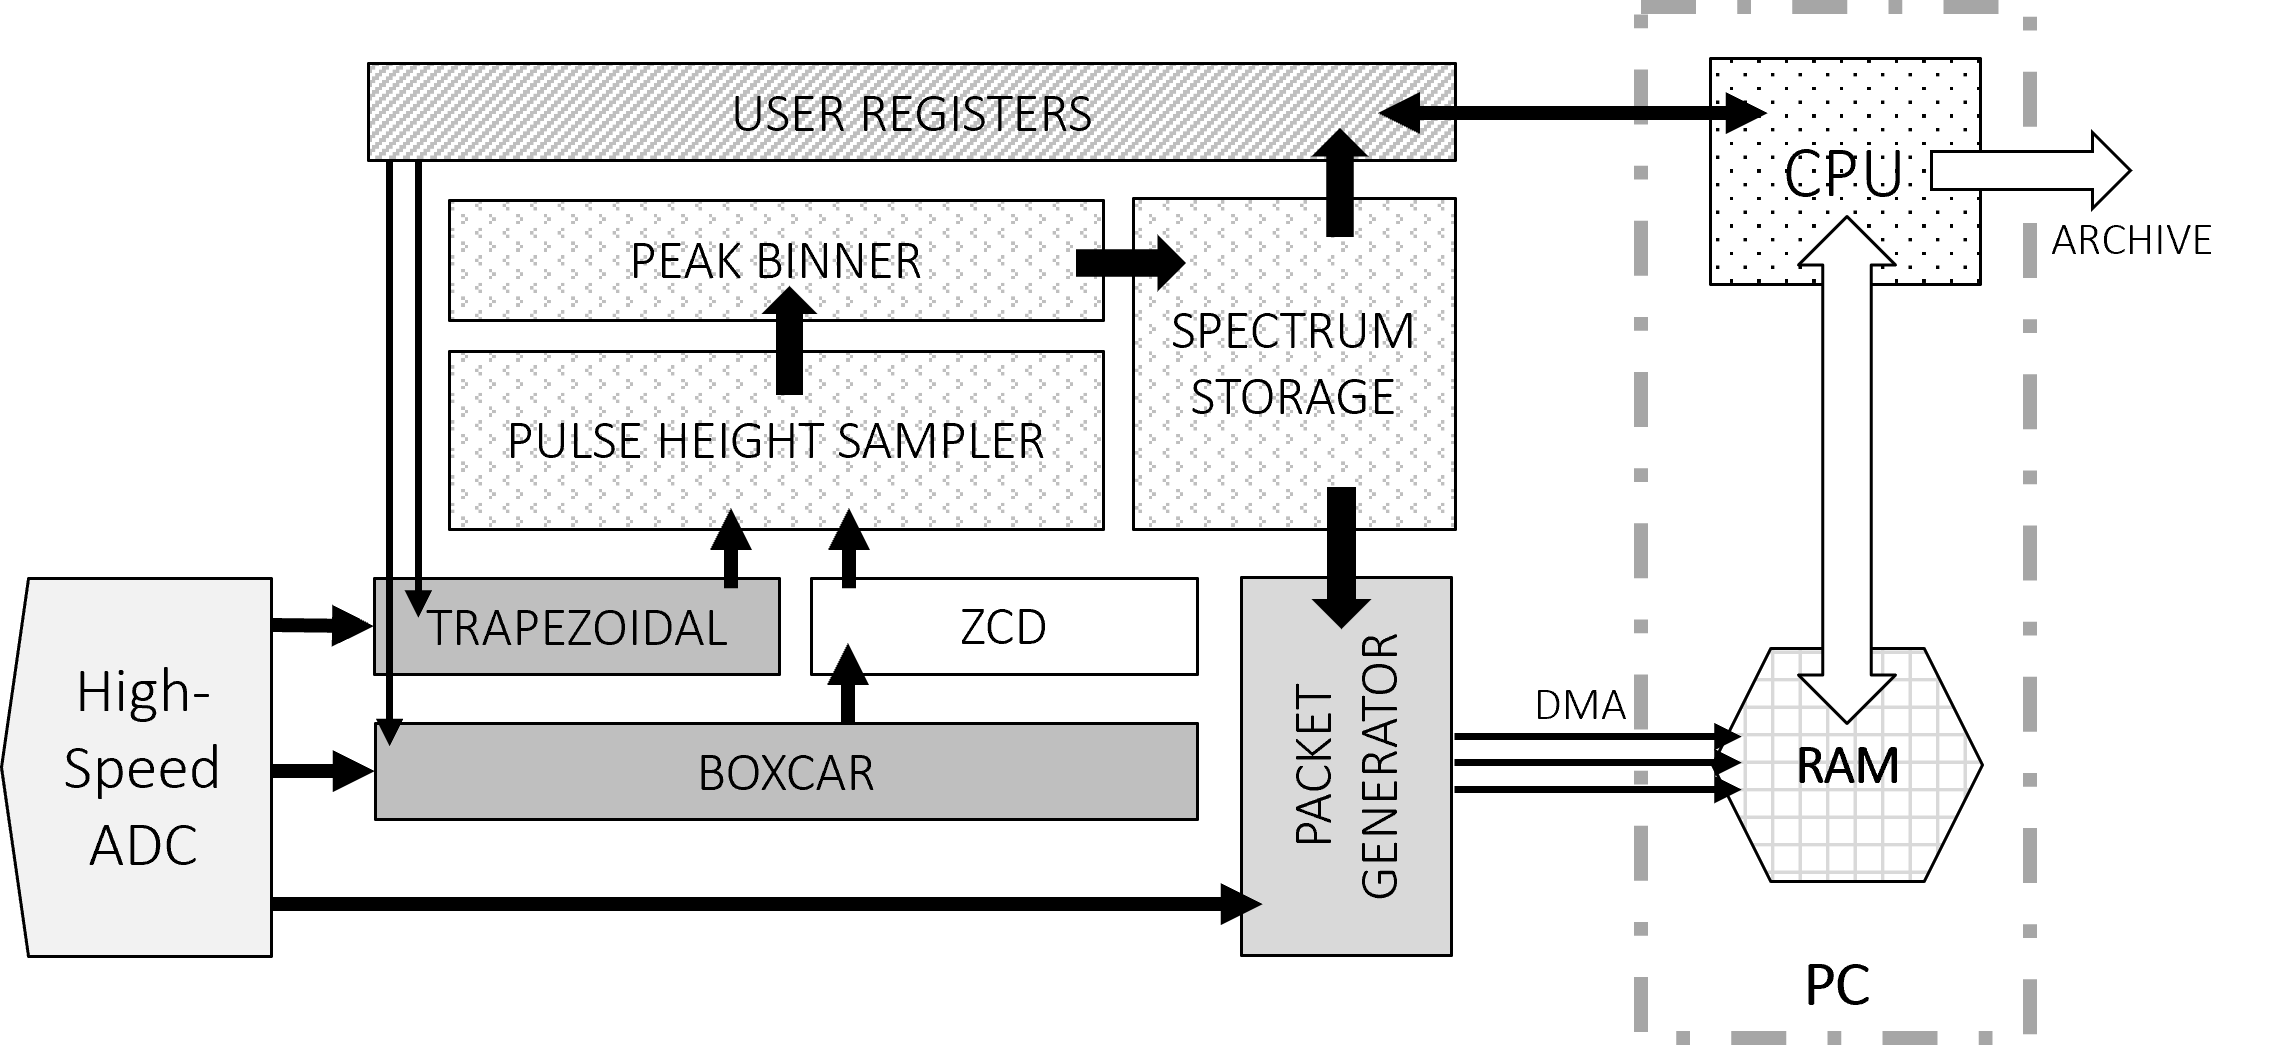
\includegraphics[width=\linewidth]{media/fpga_system_trap.png}
  \caption{Firmware overview in User Logic 2}
  \label{fig:firmware_overview} 
\end{figure}
\subsection{System control}

The system is configured and controlled through so called 
user registers. $2^{19}$ individually addressable 32-bit words
are available for reading and writing to from the PC. The first
four words are reserved for internal use. Next four have been 
dedicated for configuration and control as listed in \autoref{tab:register_control}.
The $2^{14}$ block of addresses starting from position 9, can
be used to read values from bins forming the currently held spectrum.

\subsection{Pulse detection}
Pulse detection relies on the use of a configurable boxcar filter
that then passes through a zero crossing detector. Depending on the
length of the boxcar window the result of the ZCD is delayed by an appropriate
amount so that it points to a point at which the trapezoidal filter's 
rising edge starts. To prevent false triggers the ZCD operates in two modes.
First it awaits a user specified threshold value to be crossed. Only after
that event occurs, does it start looking for a zero crossing.
After a zero crossing the system returns back to the threshold awaiting state.
\autoref{fig:zcd_algorithm} illustrates this algorithm. 
The threshold value is transferred through user registers and does not require
the FPGA to be reprogammed if modified.

\begin{figure}[H]
  \centering
  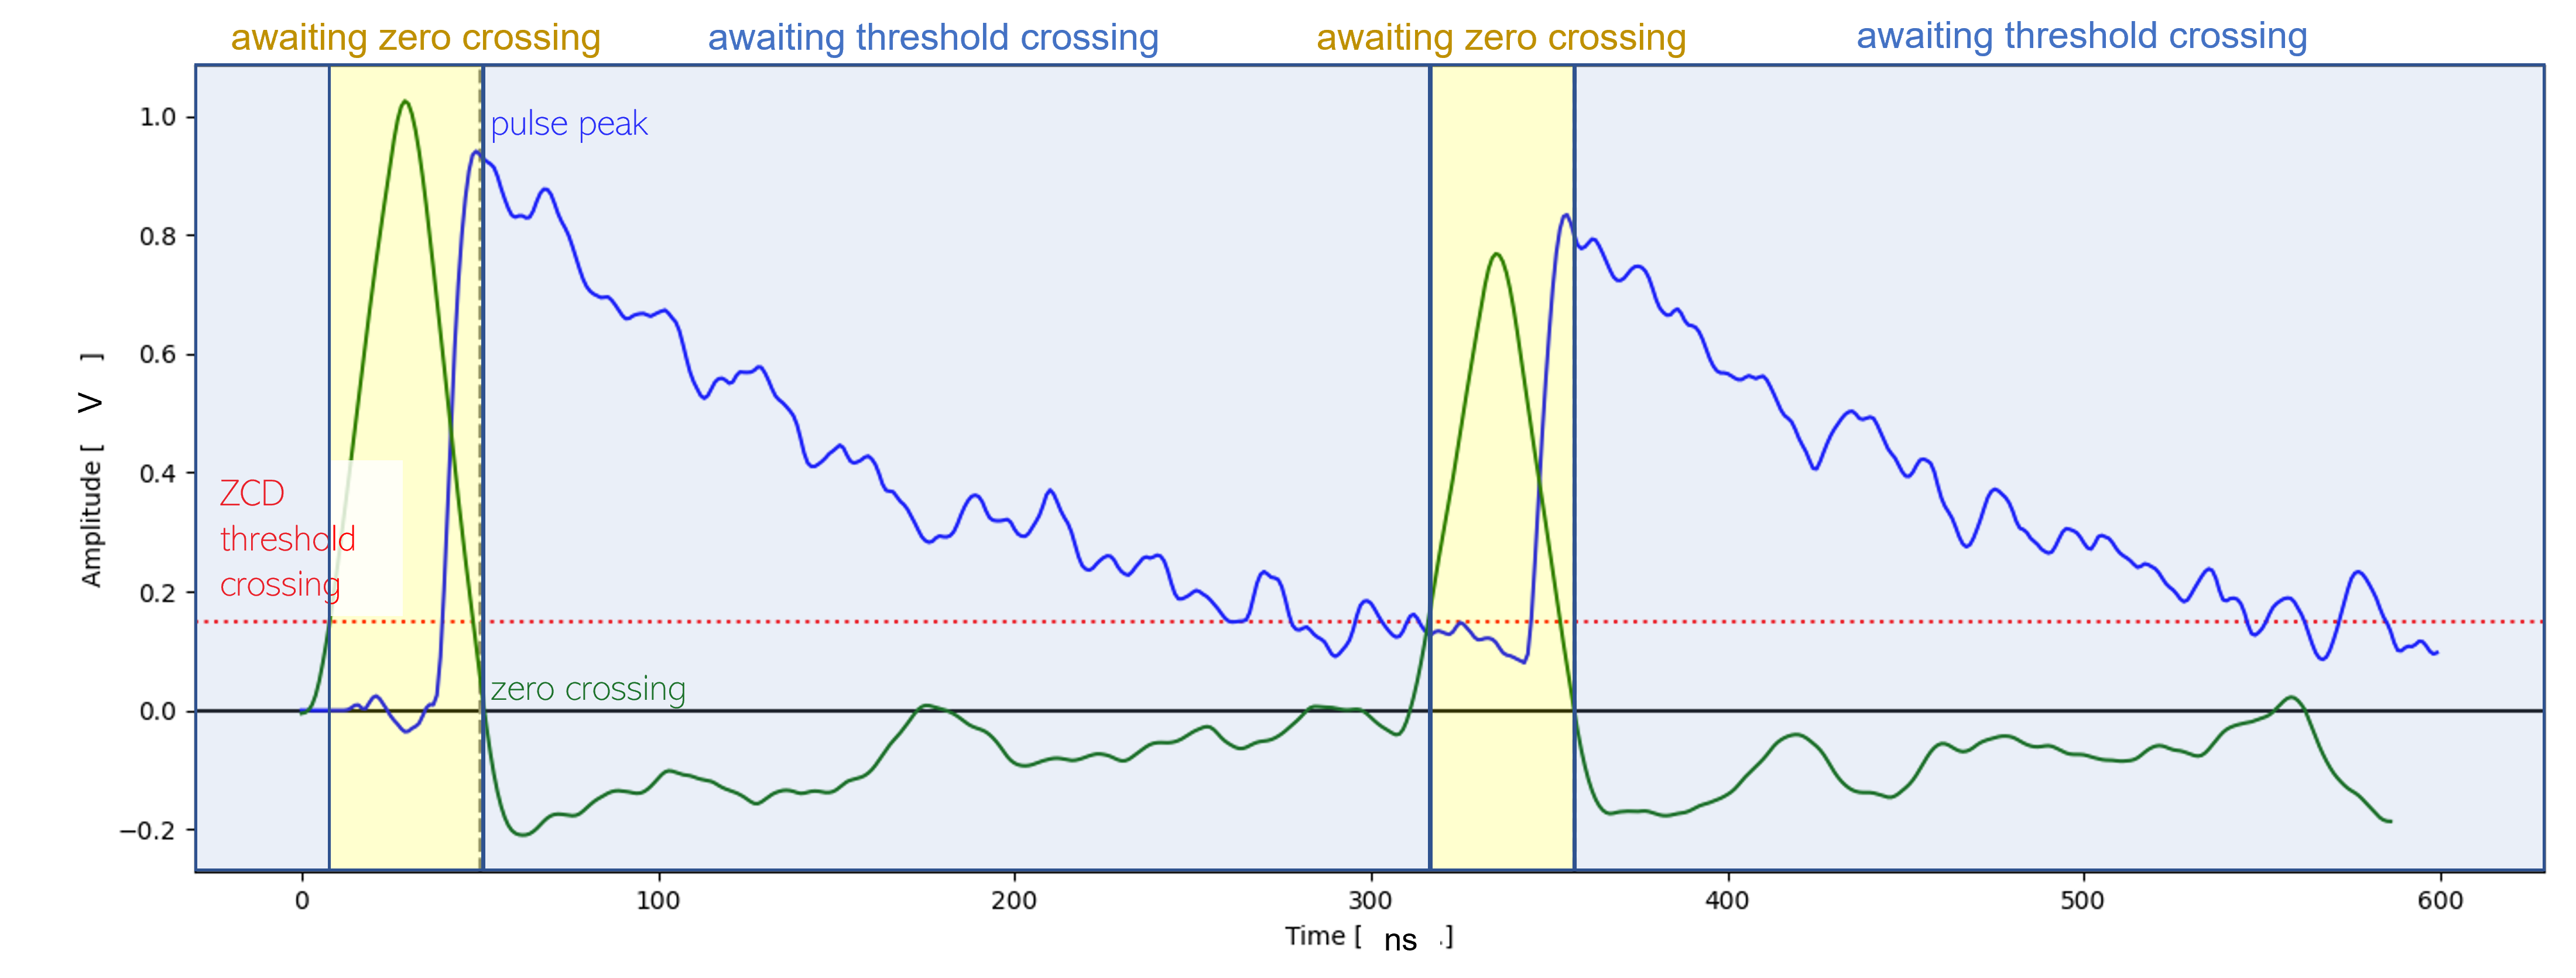
\includegraphics[width=\linewidth]{media/zcd_algorithm.png}
  \caption{Zero Crossing Detection algorithm employed in firmware for pulse detection and timing}
  \label{fig:zcd_algorithm} 
\end{figure}
\subsection{Pulse height analysis}
The timing generated by the ZCD is resynchronized to a trapezoidal filter, 
to indicate the start of a trapezoid forming. After a delay equal to the 
trapezoid edge the sampling module is triggered. The module
accumulates every sample from the trapezoid flattop and 
divides the end result by the number of samples.
The result grants an average flattop height that corresponds
to the pulse peak height. The averaging action reduces overall noise
and increases precision of the measurement.


\begin{figure}[H]
  \centering
  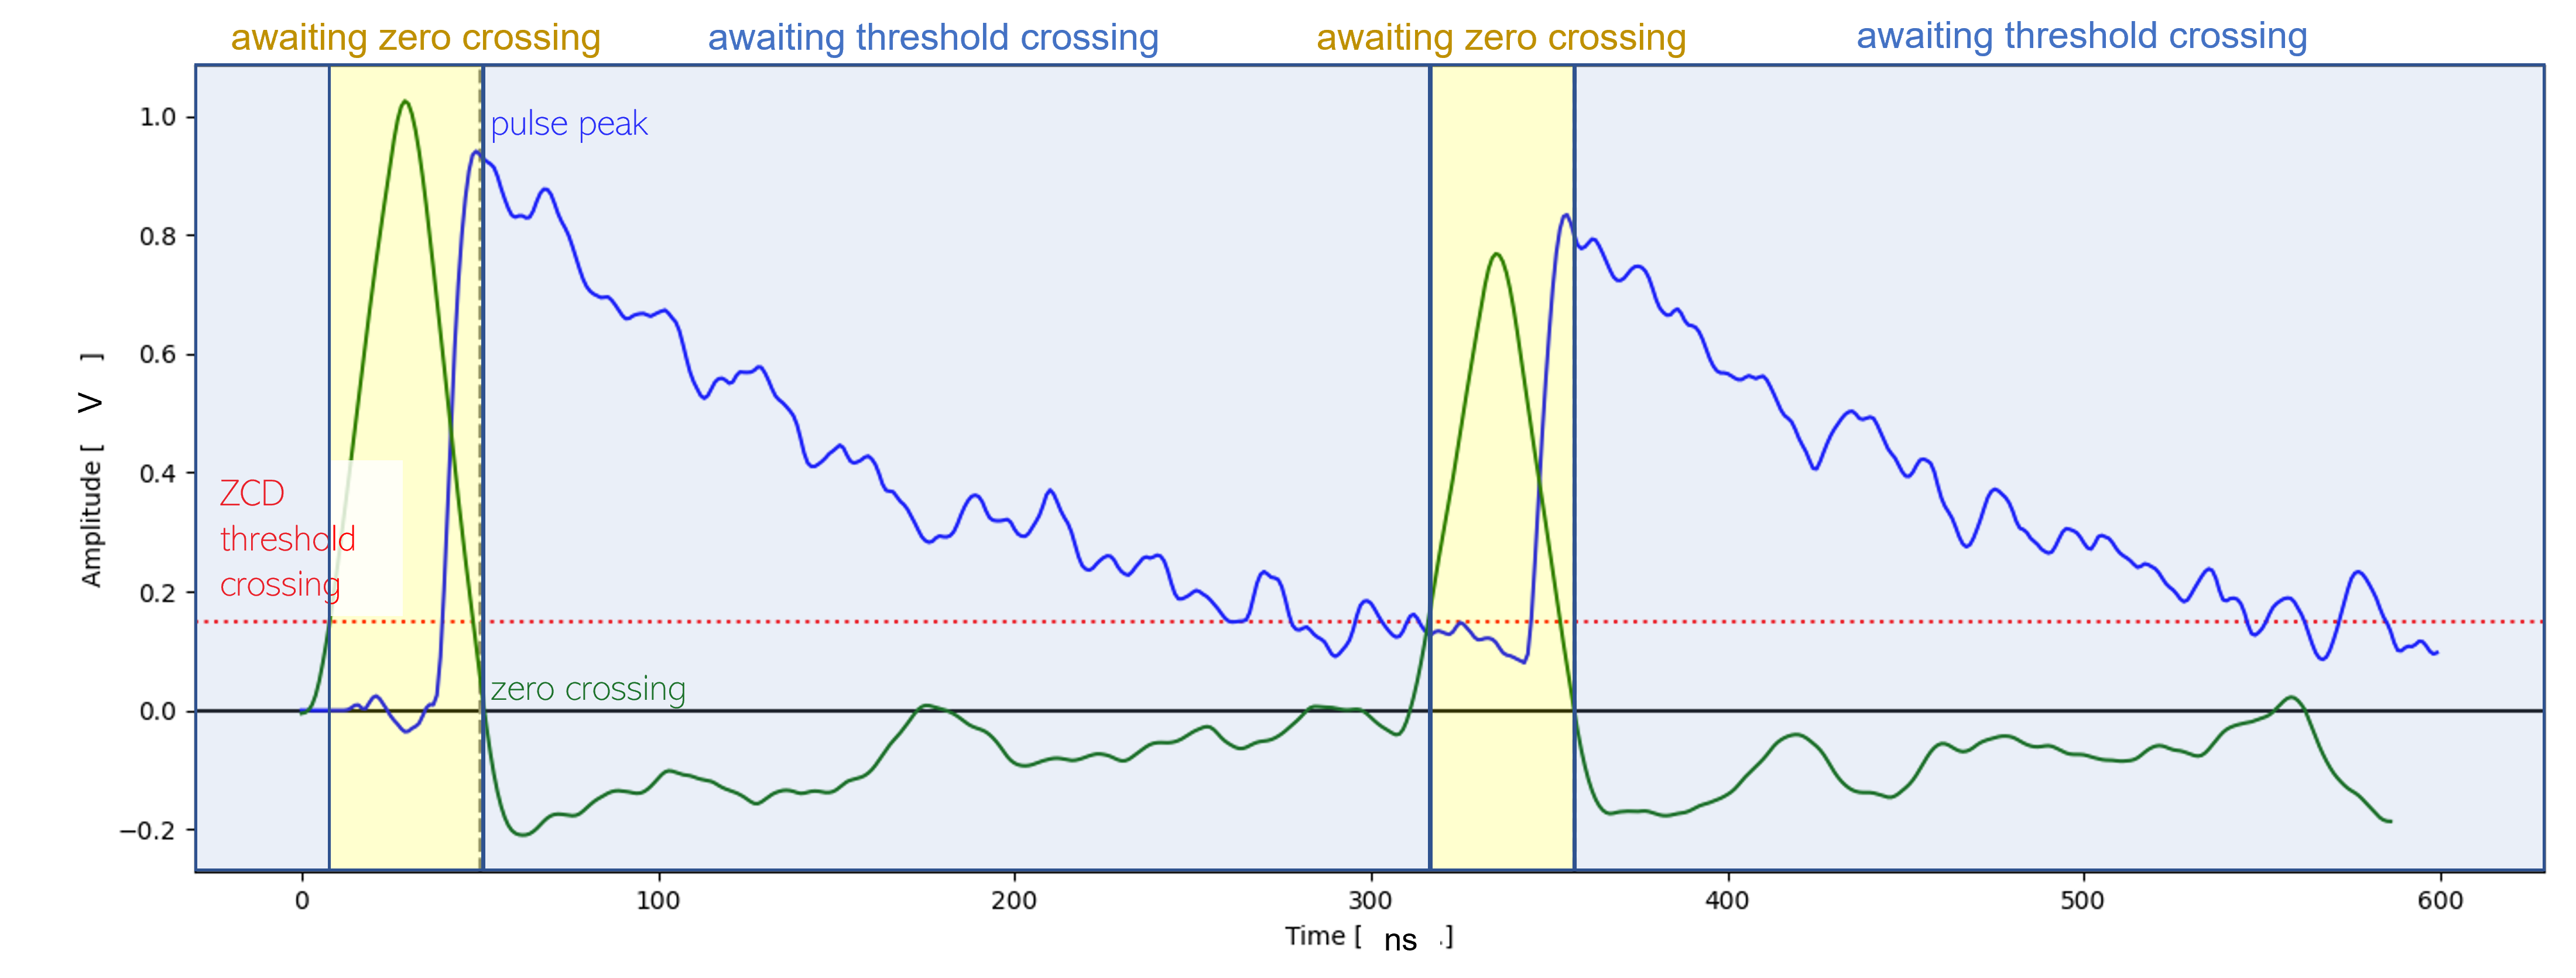
\includegraphics[width=\linewidth]{media/zcd_algorithm.png}
  \caption{Zero Crossing Detection algorithm employed in firmware for pulse detection and timing}
  \label{fig:zcd_algorithm} 
\end{figure}
\subsection{Record integrator}
\subsection{Spectrum storage and transfer}
